\chapter{Incoherency} \label{chap:Incoherency}

In this chapter the blending operator is analyzed in greater detail. Then a measure for incoherency will be introduced and the role of incoherency for deblending will be discussed.

\section{Analysis of the Blending Matrix} \label{sec:BlendingMatrix}

In order to optimize the blended acquisition design, one must understand the properties of the blending matrix $\mathbf{\Gamma}$ and its influence on the deblending performance.

The blending matrix $\mathbf{\Gamma}$ determines the pseudo-deblended data,

\begin{equation}
	\mathbf{P}_{ps} = \mathbf{P \Gamma \Gamma ^H},
	\label{eq:Ch-Theory-Pseudo-Deblended-Data}
\end{equation}

which is a superposition of the unblended data, $\mathbf{P}$, and the blending noise, $\mathbf{N}$,

\begin{equation}
	\mathbf{P}_{ps} = \mathbf{P} + \mathbf{N}.
	\label{eq:Ch-Theory-PseudoSuperposition}
\end{equation}

The more incoherent the blending noise, $\mathbf{N}$, the better it can be removed by noise filters.

In the following the effect of the blending matrix, $\mathbf{\Gamma}$, on the matrix product $\mathbf{\Gamma \Gamma}^H$ and on the pseudo-deblended data is analyzed. For simplicity, it is assumed that all sources are equal in strength and fire the same signature into the earth. This means that the blending matrix, $\mathbf{\Gamma}$, only contains phase shift terms, $\mathrm{e}^{-j \omega \Delta t}$, with an amplitude equal to 1 or 0. It is also assumed that each shot is fired only once, unlike e.g. the shot repetition case \citep{Sixue}.

Each row of $\mathbf{\Gamma}$ represents a shot $k$ and each column of $\mathbf{\Gamma}^H$ represents a shot $l$ with a complex conjugated phase term (see Figure \ref{fig:Ch-Theory-GGH}). Hence, each element $g_{kl}$ of the matrix $\mathbf{\Gamma \Gamma}^H$ is the dot product between the $k^{th}$ shot and the complex conjugate of the $l^{th}$ shot.

\begin{figure}
	\centering
	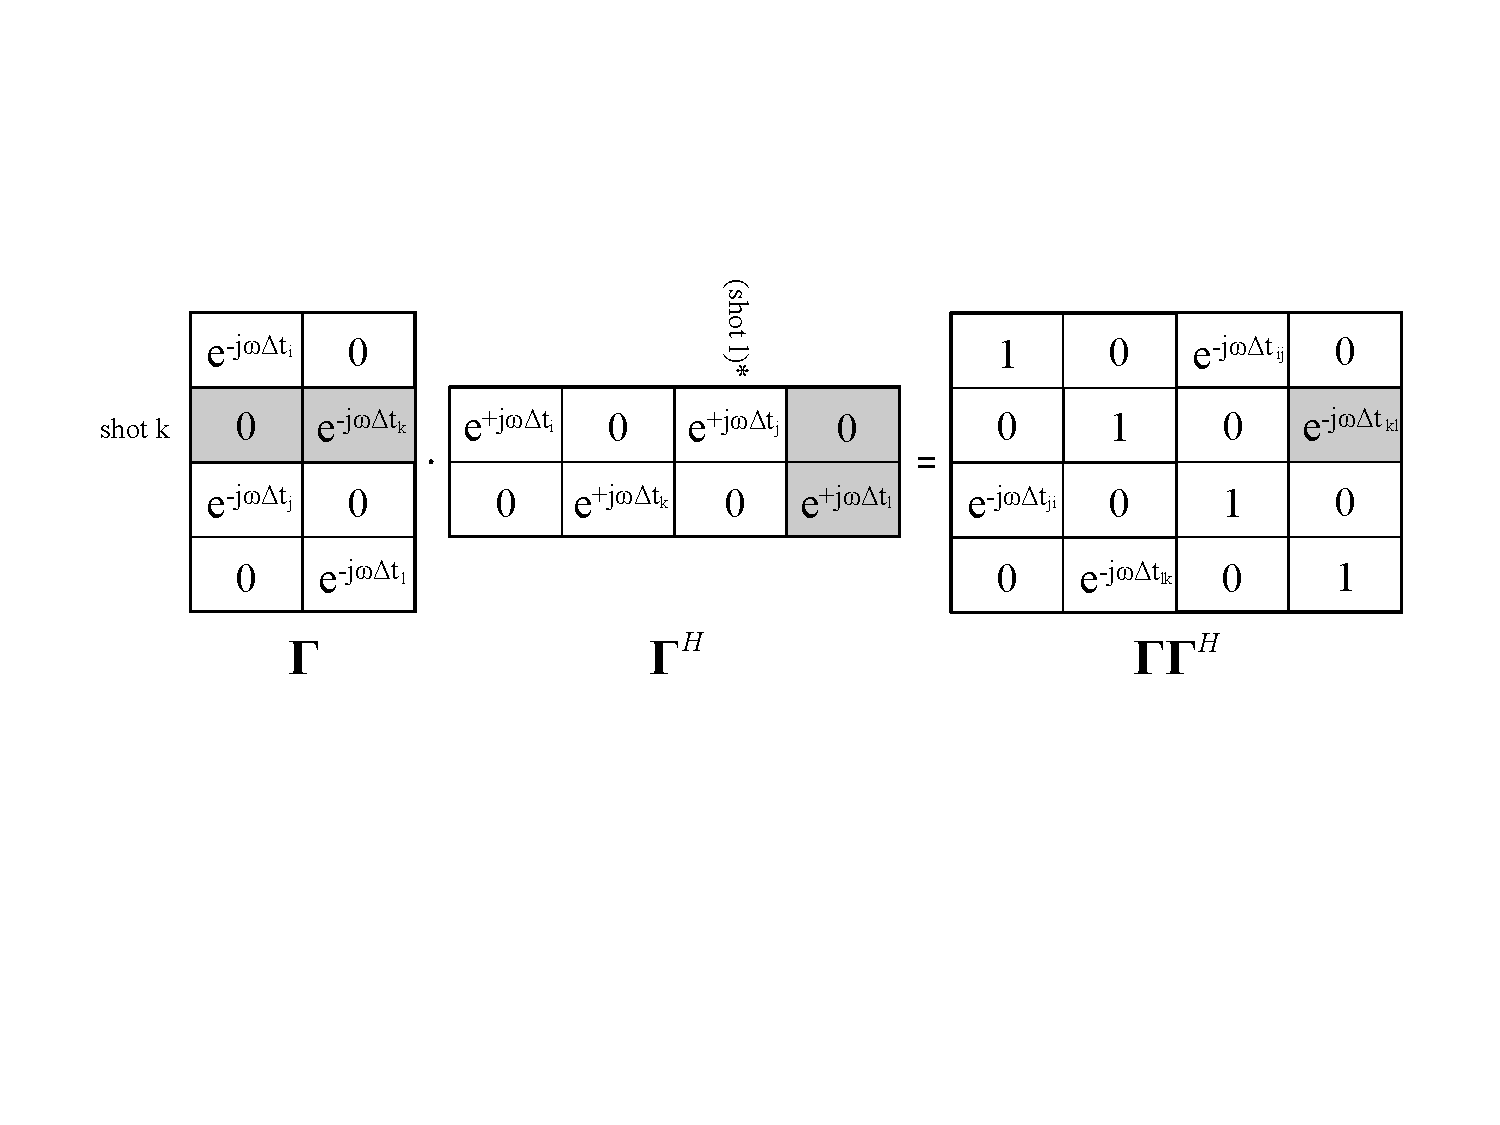
\includegraphics[width = \textwidth]{Plots/GGH}
	\caption{Illustration of the matrix product, $\mathbf{\Gamma \Gamma}^H$. In this notation $\Delta t_k$ refers to the phase shift of the source $k$, and $\Delta t_{kl}$ refers to the phase shift between the sources $k$ and $l$, $\Delta t_{kl} = \Delta t_k - \Delta t_l$.}
	\label{fig:Ch-Theory-GGH}
\end{figure}

Consequently, an element $g_{kl}$ of the product $\mathbf{\Gamma \Gamma}^H$ represents the overlap of the shot $k$ and $l$ for all experiments. The main diagonal of $\mathbf{\Gamma \Gamma}^H$ refers to the overlap of each shot with itself, which of course is perfect and therefore equal to 1. The off diagonal elements of $\mathbf{\Gamma \Gamma}^H$ are either 0 if the associated shots do not overlap, or contain a phase shift, $\mathrm{e}^{\, -j \omega \Delta t_{kl}}$.

\subsection*{Temporal incoherency}

In equation \ref{eq:Ch-Theory-Pseudo-Deblended-Data} the main diagonal elements of $\mathbf{\Gamma \Gamma}^H$ copy the data matrix, $\mathbf{P}$, while the off-diagonal elements create the blending noise, $\mathbf{N}$. In case of a coherent firing time delay the elements along a sub-diagonal $g_{ik}$ are in phase. This means that the sub-diagonal elements will shift the columns of the data matrix and apply a coherent phase shift to each of them resulting in the pseudo-deblended receiver gather shown in Figure \ref{fig:Ch-Theory-PseudoCRG-CoherentDelay}. Instead if the elements $g_{ik}$ along a sub-diagonal are out of phase, they will shift the columns of the data matrix and distort the phase of each column (see Figure \ref{fig:Ch-Theory-PseudoCRG-IncoherentDelay}). 

Figure \ref{fig:Ch-Theory-PseudoCRG-FK-CoherentDelay} and \ref{fig:Ch-Theory-PseudoCRG-FK-IncoherentDelay} display the $f$-$k$-spectra of the pseudo-blended data for constant firing time delays and random firing time delays respectively. In the case of constant firing time delays almost all of the energy maps in the signal cone. In the case of random firing time delays a significant part of the energy maps outside of the signal cone. Therefore, the coherency constraint requires random firing delays. 

In this thesis the random firing time delays are referred to as temporal incoherency.  

\begin{figure}
	\centering
	\begin{subfigure}[b]{0.3\textwidth}
		\centering
		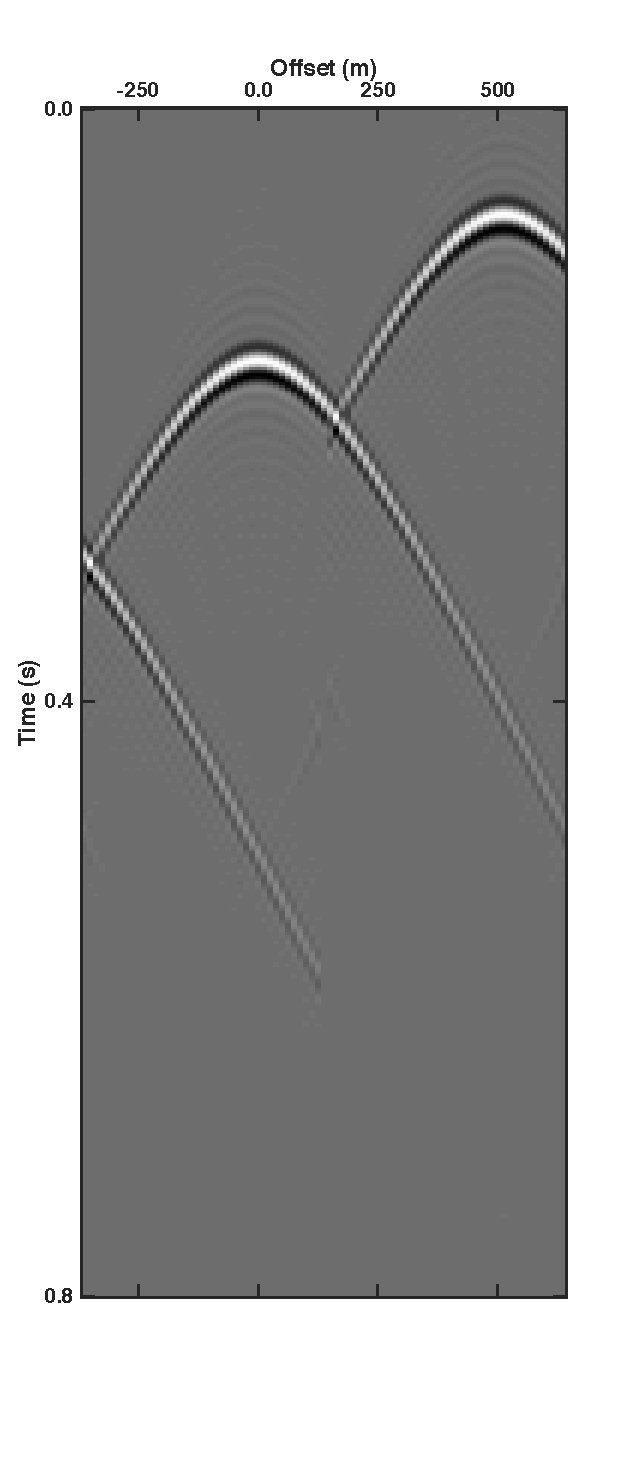
\includegraphics[width = \textwidth]{Plots/Mahdad/25iter/TimeDelay/Pseudo-DeblendedCRG_rec30_coh}
		\caption{}
		\label{fig:Ch-Theory-PseudoCRG-CoherentDelay}
	\end{subfigure}
	%
	\centering
	\begin{subfigure}[b]{0.3\textwidth}
		\centering
		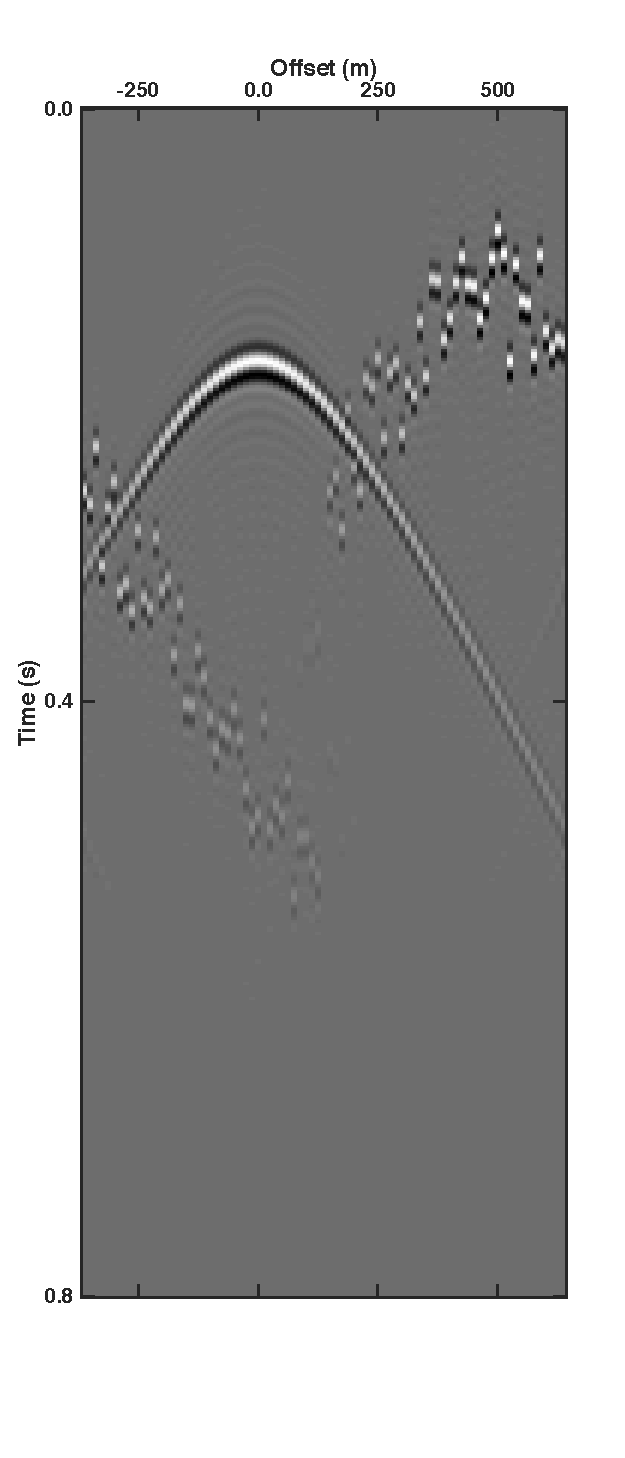
\includegraphics[width = \textwidth]{Plots/Mahdad/25iter/TimeDelay/Pseudo-DeblendedCRG_rec30}
		\caption{}
		\label{fig:Ch-Theory-PseudoCRG-IncoherentDelay}
	\end{subfigure}
	%
	\centering
	\begin{subfigure}[b]{0.3\textwidth}
	
		\centering
		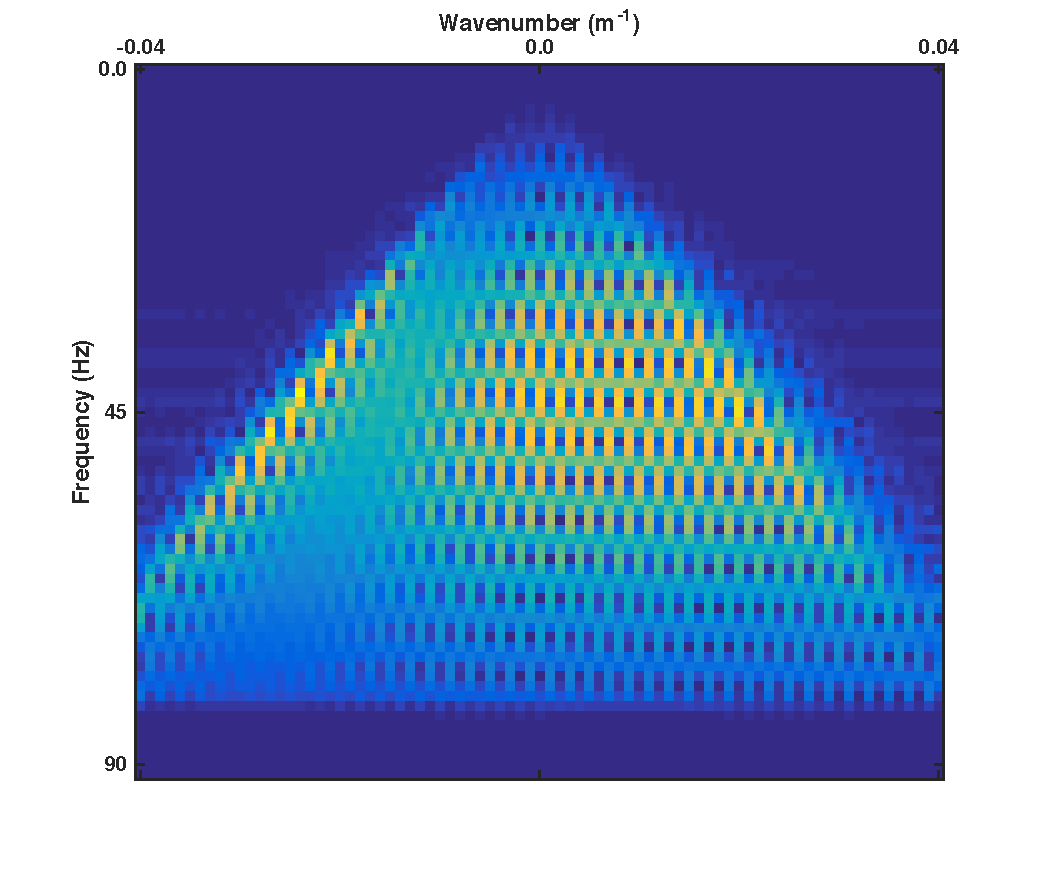
\includegraphics[width = \textwidth]{Plots/Mahdad/25iter/TimeDelay/FK-Pseudo-deblendedCRG_rec30_coh}
		\caption{}
		\label{fig:Ch-Theory-PseudoCRG-FK-CoherentDelay}
		
		\par\bigskip
		
		\centering
		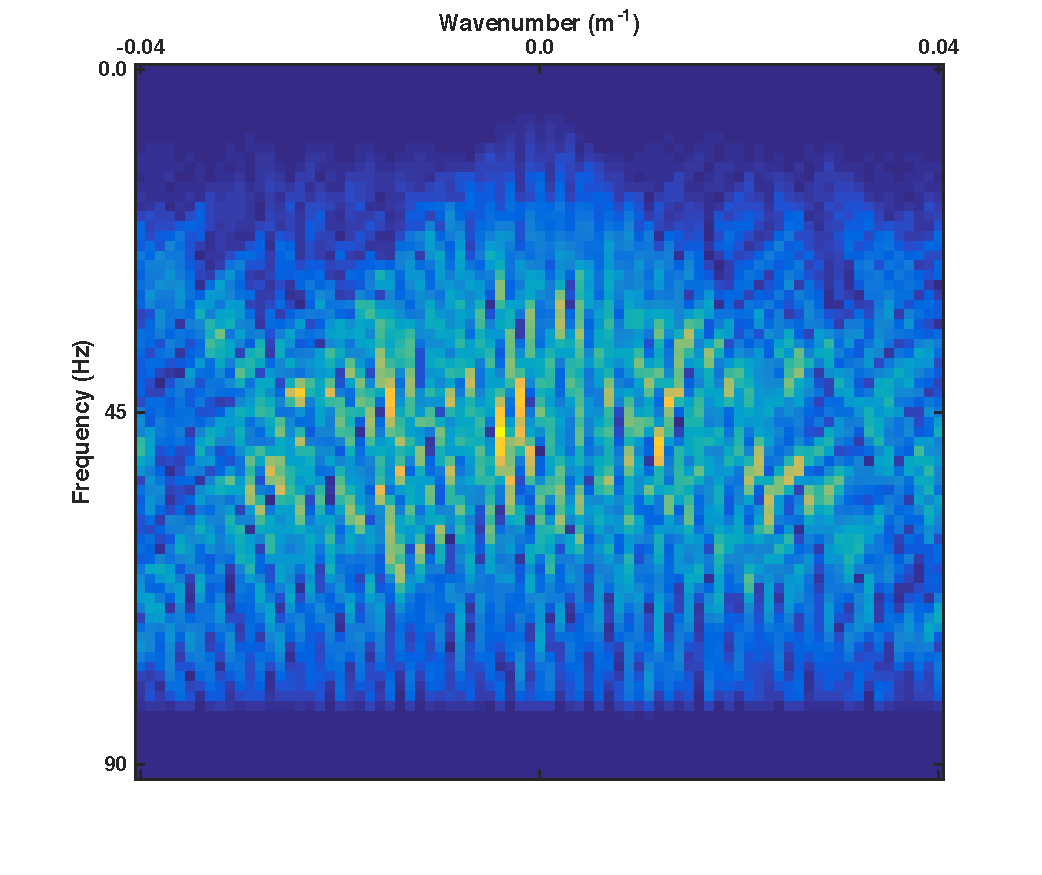
\includegraphics[width = \textwidth]{Plots/Mahdad/25iter/TimeDelay/FK-Pseudo-deblendedCRG_rec30}
		\caption{}
		\label{fig:Ch-Theory-PseudoCRG-FK-IncoherentDelay}
		
	\end{subfigure}
	
	\caption{Comparison of the pseudo-deblended receiver gather for (a) constant firing time delays of \SI{100}{\milli\second}, and (b) random firing time delays between \SI{0}{\milli\second} and \SI{100}{\milli\second}. (c) and (d) show the $f$-$k$-spectra of (a) and (b) respectively.}
	\label{fig:Ch-Theory-PseudoCRG-IncoherencyEffect}

\end{figure}

\begin{figure}
	\centering
	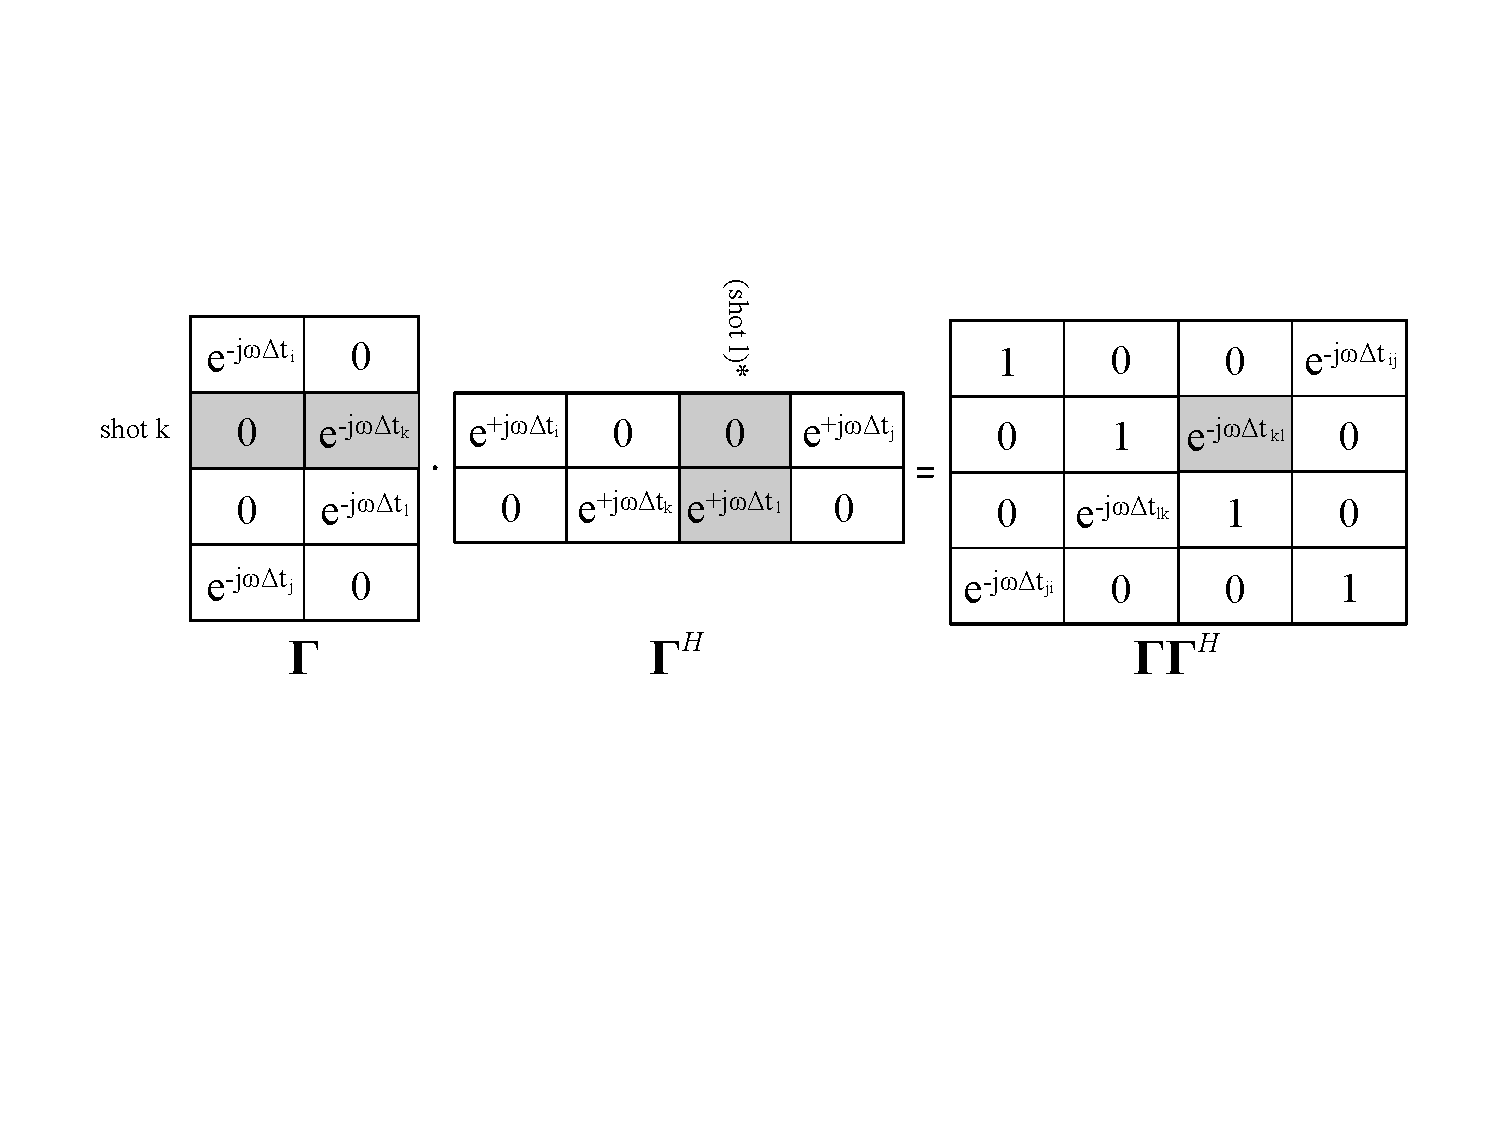
\includegraphics[width=\textwidth]{Plots/GGH_x}
	\caption{The blending matrix, $\mathbf{\Gamma}$, is obtained by interchanging the $3^{rd}$ and $4^{th}$ row of the blending matrix in Figure \ref{fig:Ch-Theory-GGH}. In acquisition this is equivalent to moving source 3 to experiment 2, and source 4 to experiment 1. A random permutation of the rows of the blending matrix spreads the off-diagonal elements of the matrix product, $\mathbf{\Gamma\Gamma}^H$. The elements are not assembled on the sub-diagonals anymore.}
	\label{fig:Ch-Theory-GGHx}
\end{figure}

\begin{comment}
In order to generate incoherent source interference, $\mathbf{N}$, it is therefore favorable if the elements $a_{ik}$ of each lower or upper diagonal are out of phase. For example, considering the $n^{th}$ upper or lower diagonal of the matrix $\mathbf{\Gamma \Gamma}^H$ this observation translates to the acquisition as follows: All source pairs, which are $n$ sources apart from each other, must be fired incoherently. The incoherent firing is realized by delaying blended sources with a random time delay.
\end{comment}


\subsection*{Spatial incoherency}

Of course, the degree of incoherency of the source interference, $\mathbf{N}$, also depends on whether the sources blended in an experiment are selected randomly, or in a spatially coherent pattern. For example, one expects the source interference to be more incoherent if in each experiment randomly picked sources are blended, than if in each experiment adjacent sources are blended (see Figure \ref{fig:Ch-Theory-GGHx}).

In 2D blending only adjacent sources can be blended, thus, the blended sources cannot be selected randomly. This changes when blending is extended to 3D: Within the crossline direction sources can be selected randomly and blended. 

\todo[inline]{This might need some extra explanation and plot!}

\begin{comment}

In terms of the blending matrix $\mathbf{\Gamma}$ a spatially incoherent firing pattern means that the rows, i.e. the sources, are shuffled randomly. As a consequence the off-diagonal elements of the matrix product $\mathbf{\Gamma \Gamma}^H$ are reordered randomly. This shuffling process can help to further distort the phase of the interfering sources. However, if the maximum allowed time delay between blended sources is aready large the spatially incoherent blending pattern will not increase the incoherency of the interfering sources.   

In practice, the maximum allowed firing time delay is limited by the available acquisition time. The spatial distribution of blended sources is constraint by the acquisition design.
	
\end{comment}


\FloatBarrier


